\begin{figure}[t]
\centering
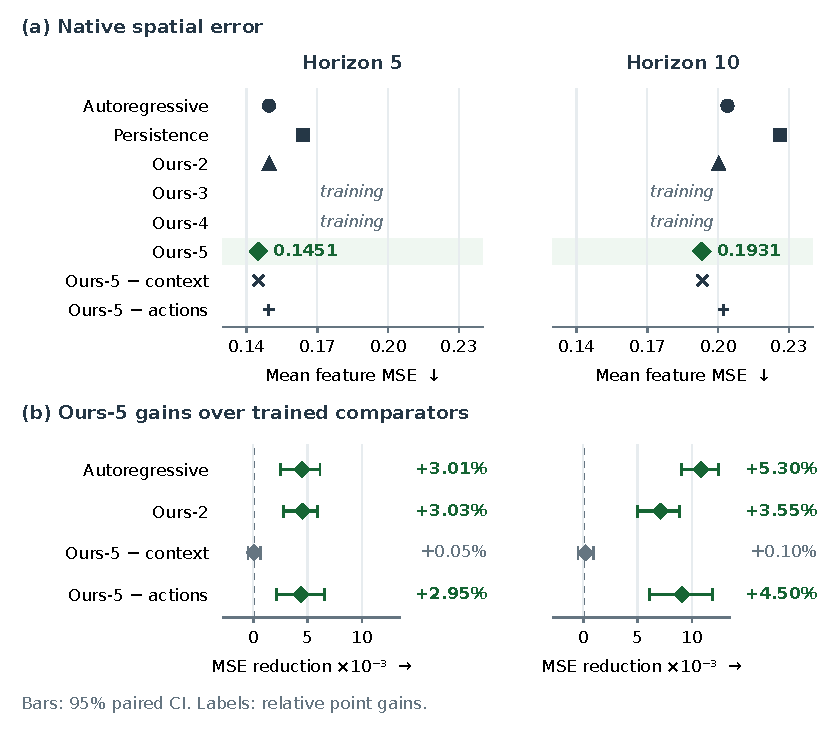
\includegraphics[width=\linewidth]{generated/real_video/spatial_versions_comparison.pdf}
\caption[Spatial versions and paired improvements.]{Completed spatial versions on original DROID validation. (a) Absolute native 4$\times$4 standardized feature MSE at endpoints 5 and 10; green marks identify our mechanism variants, not a winner. (b) Ours-5 is the reference for paired reductions against six comparators; right of zero favors Ours-5. Only registered matching contrasts are used. Ours-4 and Ours-5 are close: both native comparison intervals include zero, and Ours-4 has the lower h5 point estimate. Bars show 95\% paired recording-session $\times$ training-seed bootstrap intervals (10,000 draws; seed 173); percentages are relative point reductions. Gray intervals include zero; favorable green intervals exclude zero without multiplicity adjustment. All 21 spatial models completed 30 epochs: 15 original models plus 6 new component models; the four-arm factorial subset has 12 models including reused controls. Ours-3/4 were added in a registered follow-up after the original controls were revealed. Evaluation uses 1,631 matched windows, 141 episodes, 59 sessions and 3 seeds. Windows are averaged within episodes, then episodes and seeds equally. Ours-1 has a different protocol and remains off this axis. Companion tables preserve the original 16 comparisons and all 20 component effects, including four signed interactions and every unfavorable or inconclusive result. These are development comparisons, not independent-test or state-of-the-art claims.}
\label{fig:spatial-versions}
\end{figure}
